% Chapter Template

\chapter{System Design and Development} % Main chapter title

\label{Chapter4} % Change X to a consecutive number; for referencing this chapter elsewhere, use \ref{ChapterX}

\lhead{Chapter 4. \emph{System Design and Development}} % Change X to a consecutive number; this is for the header on each page - perhaps a shortened title

%----------------------------------------------------------------------------------------

\section{Introduction}

This chapter will focus on the requirements that the proposed solution must fulfil, outline the challenges involved and highlight the key technologies that will be used.


%----------------------------------------------------------------------------------------

\section{User Requirements}

With the research showing areas that could be focused on to improve user satisfaction, a list of proposed user requirements was  created to identify specific features that would improve the user experience. The following list shows the final requirements for proposed solution:

\subsection{Login System}

A login system used to hold the patients identity and allow them to easily manage their appointments on multiple devices. This will also act as a security mechanism to ensure that medical information is only revealed to the patient in question.

\subsection{List of Appointments}

A list of the patients appointments which is kept up to date and updated automatically when changes are made. This will display very basic information about each appointment, such as when it occurs and the type of appointment it is.

\subsection{Appointment Information}

Tapping on an appointment in the appointment list will bring up relevant information about that appointment, including the doctor's name, location (using a map) and time. It will also include a short description about the appointment, links to useful information and contact details for emergencies.

\subsection{Appointment Notifications}

The smart device, after the patient has logged in, will listen for notifications from the server, which contain short messages that displays up-to-date information related to appointments. 

Use cases for this feature include time-based reminders so that the patient does not forget, or changes to the patients appointment such as a different location or doctor.

\subsection{Scheduling Appointments}

Although appointments are initially set-up by a healthcare professional, patients will have control over the timing of the appointment. 

The patient will tap an existing appointment, and choose to schedule or re-schedule it. They will be able to post a time window that they want the appointment to occur within, and the server will respond with 3 choices. 

The patient will then be able to either confirm one of the choices, or alter their timing window.

%----------------------------------------------------------------------------------------

\section{System Requirements}

Alongside the user requirements, a list of system requirements was also created to support the user requirements and ensure the solution is flexible under possible future requirement changes. Here is the finalised list of system requirements:

\subsection{Cross-Platform}

Running on multiple devices is important so that the usability of the service is maximised. Although this project will only target the Android platform, it will be designed such that it can be easily adapted to run on alternate devices such as iOS and web-browsers.

\subsection{Representational State Transfer (Restful) Web Services}

Because scheduling is a complex problem, the solution needs to be easily integrable with other systems. Multiple endpoints will be available through restful web services, so that components of the system can be easily utilised by other systems. 

For example, many scheduling solutions already exist, written in different programming languages and implemented in different ways. The system should be designed in a way that it can easily 'plug-in' to these scheduling solutions and utilise them fully through restful web-services.

\subsection{One Development Language}

Very few devices share development languages, which can make it troublesome to offer cross platform support.

For the sake of simplicity and given the time requirements, this project will also aim to implement the server and client in the same programming language, C\#.

%----------------------------------------------------------------------------------------

\section{Development and Technology Used}

To fulfil all user and system requirements, various technologies will be used. Here, I will give a brief description of each technology and what role it will play in the proposed solution.

\subsection{Mono and Xamarin}

Mono is an open source implementation of the C\# programming language that is cross-platform. This allows development of C\# code that can be compiled and run on Windows, Linux and Mac systems.

Xamarin is a mobile app development framework built on Mono, targeting the Android, iOS and Windows Phone platforms. Also, because Xamarin is written using C\#, it can integrate easily with the Windows SDK for the development of Windows Desktop Applications. 

Xamarin allows business layer logic to be shared across the different platform implementations, essentially having one main code-base rather than a seperate one for each platform.

\begin{figure}[htbp]
	\centering
		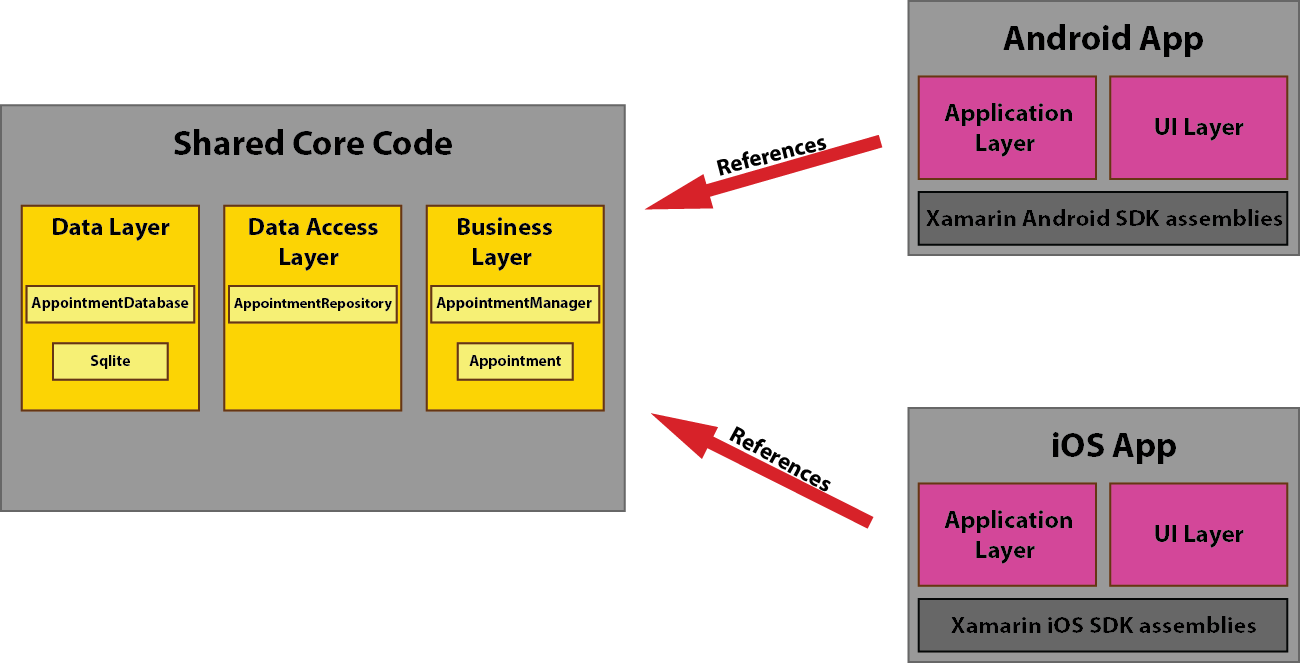
\includegraphics[width=\textwidth,height=\textheight,keepaspectratio]{Figures/AppOverview.png}
		\rule{35em}{0.5pt}
		\caption[Diagram showing client architecture and business logic being reused across multiple platforms]{Diagram showing client architecture and business logic being reused across multiple platforms}
	\label{fig:appoverview}
\end{figure}

The server application will therefore be written in C\# with the possibility of being compiled using Mono, allowing it to run on either Windows or Linux server machines (although this is beyond the scope of this project). The Android App will also be written in C\# using the Xamarin framework, allowing the code-base to be easily integrated with future platforms.

\subsection{Communication}

The system requires two types of communication based on the requirements, urgent and direct. It is very important to differentiate between these two when targeting mobile devices, due to the following issues:
\begin{itemize}
	\item Bandwidth is limited
	\item Devices aren't always online
	\item Connections are unreliable
	\item Constant communication can cause excessive power consumption
\end{itemize}

Due to these issues, a constant connection to a remote server is not possible for long periods of time. This means that the communication must be separated into two separate components, each being useful for different scenarios.

\subsubsection{Push Communication}

Notification messages, also known as push notifications, are a way of sending a short notification message to a device. This is useful for sending urgent messages when the application is not being used, prompting the user for input.

There are however, limitations of this type of communication:

\begin{itemize}
	\item Only small messages are allowed to be sent
	\item The server does not know when the message has been received
	\item Server to client messages only
\end{itemize}

Push communication can be seen as a 'answering machine service'. The server leaves a short message for the device to be received at some point in the future. If the device is offline, it will receive the message as soon as it comes online again, making it a good system for unreliable connections.

Push notifications should be kept short and only contain enough data to notify the application that it needs to connect to the server for more information.

Due to these limitations, the system will only use push notifications for the following scenarios:

\begin{itemize}
	\item A sooner appointment is available for the patient
	\item An appointment has been cancelled and/or needs rescheduling
	\item Information about an appointment has been changed
\end{itemize}

'Google Cloud Messaging (GCM)' is the Android service for sending push notifications which this project will be using. It has a message limit of 4kb and is a free service, however it has a daily fair-usage limitation on how many notifications can be sent from a single application.

\begin{figure}[htbp]
	\centering
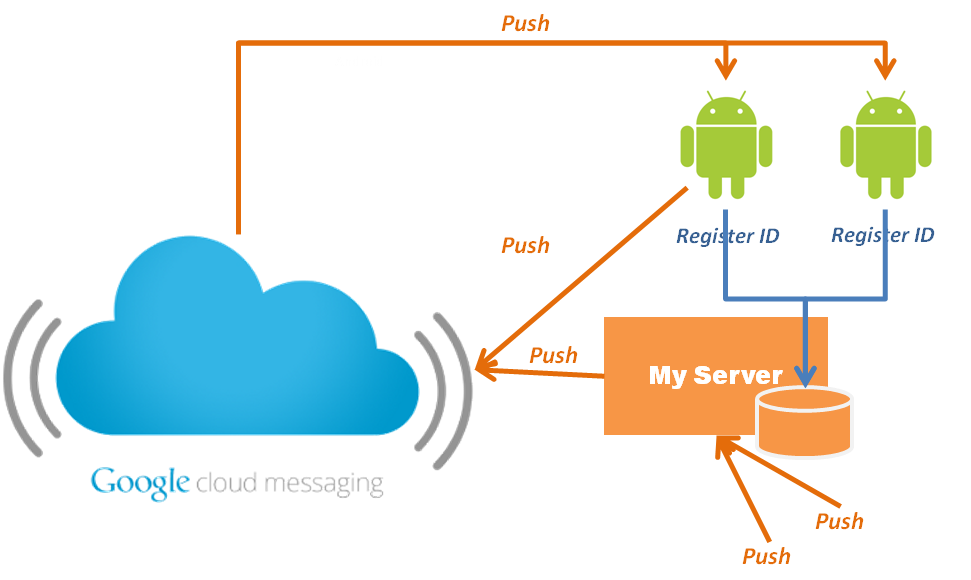
\includegraphics[width=10cm,height=10cm,keepaspectratio]{Figures/gcm.png}
		\rule{35em}{0.5pt}
	\caption[Google Cloud Messaging - \cite{gcm}]{Google Cloud Messaging - \cite{gcm}}
	\label{fig:gcm}
\end{figure}

By using this service, messages are queued and sent to the device as soon as it is available, prompting the user of some kind of notification relating to the application.

\subsubsection{Direct Communication}

After a notification has been received, or simply through using the applications features, the device will require direct communication with the server. It will require communication to:

\begin{itemize}
	\item Create or Reschedule an appointment.
	\item Request information about an appointment
	\item Request reminders about an appointment
	\item Requesting the database encryption key
\end{itemize}

All of these direct communication services will be done using restful web-service requests.

\begin{figure}[htbp]
	\centering
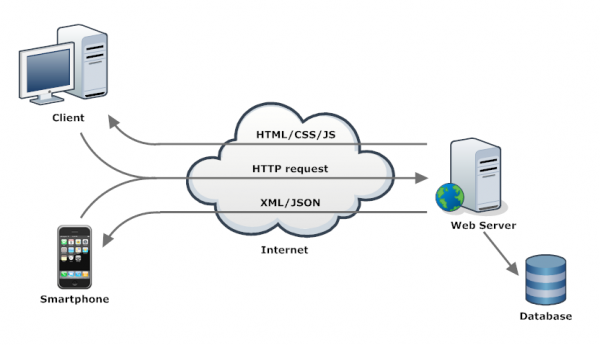
\includegraphics[width=10cm,height=10cm,keepaspectratio]{Figures/rest.png}
		\rule{35em}{0.5pt}
	\caption[RESTful Web Services cross-platform communication - \cite{rest}]{RESTful Web Services cross-platform communication - \cite{rest}}
	\label{fig:rest}
\end{figure}

Rest requests can be consumed by almost any programming language and internet accessible device. Data is translated into a mark-up language (JSON will be used for this project), transported via web-services and then reassembled on the target device.

To service these requests, the system will use 'ASP.Net'.

\subsubsection{Asp.Net}

'Asp.Net' is a MVC based web application framework for web development in C\#. It allows the binding of restful endpoints to business logic extremely easy, with built in authentication support and custom attributes to define specific restful behaviours.

\begin{figure}[htbp]
	\centering
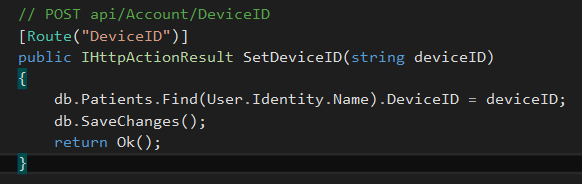
\includegraphics[width=10cm,height=10cm,keepaspectratio]{Figures/asp_example.png}
		\rule{35em}{0.5pt}
	\caption[Example of an Asp.Net web service definition]{Example of an Asp.Net web service definition}
	\label{fig:asp}
\end{figure}

The figure above shows a method that allows a smart-phone device ID to be registered to a patient's account. This particular method is for use in push notifications, so that the notifications server knows which device to send the patients notifications to. Asp.net will bind this method to the commented url above it by using the 'Route' attribute and the current controller that the method is defined in (the account controller).

%----------------------------------------------------------------------------------------

\subsection{Data Storage}

Appointment data will be stored in a SQL database, requiring relational models to be created for the solution. The finalised models will be discussed in the implementation chapter.

To create and manage the database, the system will use C\#'s 'Entity Framework'

\subsubsection{Entity Framework}

'Entity framework (EF)' is an object-relational mapper that allows developers to work easily with relational data using domain specific objects. This eliminates the need for data access code such as SQL queries, and the database can be easily designed using standard C\# code.

%----------------------------------------------------------------------------------------